\documentclass[aspectratio=169, table]{beamer}
\usepackage[utf8]{inputenc}
\usepackage[T1]{fontenc}
\usepackage{graphicx}
\usepackage{fontspec}
\usepackage{xcolor}
\usepackage{tcolorbox}
\usepackage{listings} % Add the listings package
\usepackage{hyperref} % Add the hyperref package

\lstdefinelanguage{JavaScript}{
    keywords={function, var, let, const, if, else, for, while, return, true, false},
    keywordstyle=\color{blue}\bfseries,
    ndkeywords={class, export, boolean, throw, implements, import, this},
    ndkeywordstyle=\color{orange}\bfseries,
    identifierstyle=\color{black},
    sensitive=false,
    comment=[l]{//},
    morecomment=[s]{/*}{*/},
    commentstyle=\color{gray}\ttfamily,
    stringstyle=\color{green}\ttfamily,
}

\lstset{
    breaklines=true,
    language=JavaScript,
    % ... (other style settings)
}

\lstdefinelanguage{PHP}{
    keywords={class, function, echo, if, else, foreach, for, while, return},
    keywordstyle=\color{blue}\bfseries,
    ndkeywords={public, private, protected, static},
    ndkeywordstyle=\color{purple}\bfseries,
    identifierstyle=\color{black},
    sensitive=false,
    comment=[l]{//},
    morecomment=[s]{/*}{*/},
    commentstyle=\color{gray}\ttfamily,
    stringstyle=\color{green}\ttfamily,
}

\lstset{
    breaklines=true,
    language=PHP,
    % ... (other style settings)
}

\setsansfont[
  ItalicFont=fonts/TitilliumWeb-Italic.ttf,
  BoldFont=fonts/TitilliumWeb-Bold.ttf,
  BoldItalicFont=fonts/TitilliumWeb-BoldItalic.ttf,
]{TitilliumWeb-Regular.ttf}

\subtitle{IF140303 Web-based Application Development}
\title{\Huge {\textbf{10: \\Resful API}}}
\date[Serial]{\scriptsize {PRU/SPMI/FR-BM-18/0222}}
\author[Pradita]{\small {\textbf{PRADITA UNIVERSITY}}}

\usetheme{Pradita}

\begin{document}
\begin{frame}
    \titlepage
\end{frame}

\begin{frame}{Goals - Restful API Laravel}
\vskip1cm
    \begin{itemize}
        \item To understand the concept of RESTful APIs and their importance in web development
        \item To learn how to create RESTful APIs using the Laravel framework
        \item To explore the different HTTP methods (GET, POST, PUT, DELETE) and their significance in API design
        \item To implement CRUD (Create, Read, Update, Delete) operations using RESTful routes and controllers in Laravel
        \item To gain practical experience in building a complete RESTful API with Laravel and testing it using tools like Postman
        \item To grasp the concepts of authentication and security considerations when developing APIs
    \end{itemize}
\end{frame}

\begin{frame}{Introduction to Restful API}
    \vskip1cm
    \begin{itemize}
        \item RESTful API stands for Representational State Transfer Application Programming Interface.
        \item It's an architectural style that defines a set of constraints for creating web services.
        \item RESTful APIs are designed to be scalable, stateless, and easy to consume by various clients.
        \item They use standard HTTP methods like GET, POST, PUT, and DELETE to perform actions on resources.
        \item REST APIs follow a client-server model where clients request resources, and servers respond with data.
        \item Resources are identified by URLs, and data can be sent and received in various formats like JSON or XML.
    \end{itemize}
\end{frame}

\begin{frame}[fragile]{Set Up Converter Apps}
    \begin{itemize}
        \item create a Models in Models Folder Converter.php
        \item create a file in Model folder called converters.json
        \item (in CMD) php artisan make:request Converter/StoreConverterRequest
        \item (in CMD) php artisan make:request Converter/UpdateConverterRequest
        \item (in CMD) php artisan make:controller API/ConverterController --resource
    \end{itemize}
\end{frame}

\begin{frame}[fragile]{Set Up Converter Apps}
    \begin{itemize}
        \item create a Models in Models Folder Converter.php
        \item create a file in Model folder called converters.json
        \item (in CMD) php artisan make:request Converter/StoreConverterRequest
        \item (in CMD) php artisan make:request Converter/UpdateConverterRequest
        \item (in CMD) php artisan make:controller API/ConverterController --resource
    \end{itemize}
\end{frame}

\begin{frame}[fragile]{Custom Response (Advanced)}
    \begin{itemize}
        \item Create a file named \texttt{ResponseMacroServiceProvider.php} in the \texttt{Providers} folder.
        \item This file contains a function to define your own custom response for your RESTful API.
        \item This approach is highly useful as the defined function can be reused across your application.
        \item Register this service provider in the \texttt{config} folder, specifically in the \texttt{app.php} file, under the \texttt{providers} section by adding \texttt{App\textbackslash Providers\textbackslash ResponseMacroServiceProvider::class}.
        
    \end{itemize}
\end{frame}

\begin{frame}[fragile]{Custom Response (Advanced)}
    \begin{itemize}
\item The \texttt{api} function will be part of our custom response (details in the next slide).
        \item Example usage:
        \begin{lstlisting}[language=PHP]
return response()->api(null, 'Currency converter deleted successfully', null, Response::HTTP_OK);
        \end{lstlisting}
    \end{itemize}
\end{frame}


\begin{frame}[fragile]
 \frametitle{ResponseMacroServiceProvider.php}
 \vskip1cm
 \begin{center}
  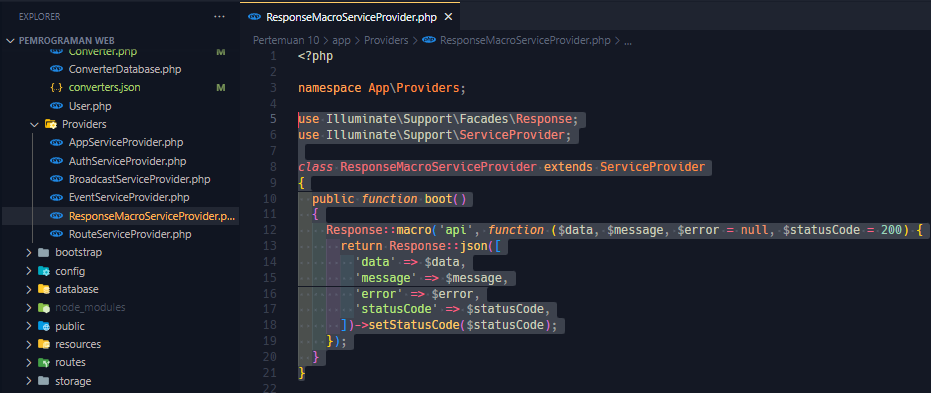
\includegraphics[width=0.8\textwidth]{classFiles/pertemuan-10-custom-response.png}
 \end{center}
\end{frame}

\begin{frame}[fragile]{Handling Request in Laravel}
    \begin{itemize}
        \item You can create validation based on \texttt{'key' => 'rules'} syntax.
        \item In Laravel, there are various rules available, such as \texttt{'required'} for ensuring a value is not null, \texttt{'string'} for validating a string, \texttt{'numeric'} for validating numeric values, and more.
        \item You can explore more about these rules in the Laravel documentation: \url{https://laravel.com/docs/10.x/validation#available-validation-rules}
    \end{itemize}
\end{frame}

\begin{frame}[fragile]
 \frametitle{StoreConverterRequest.php}
 \vskip1cm
 \begin{center}
  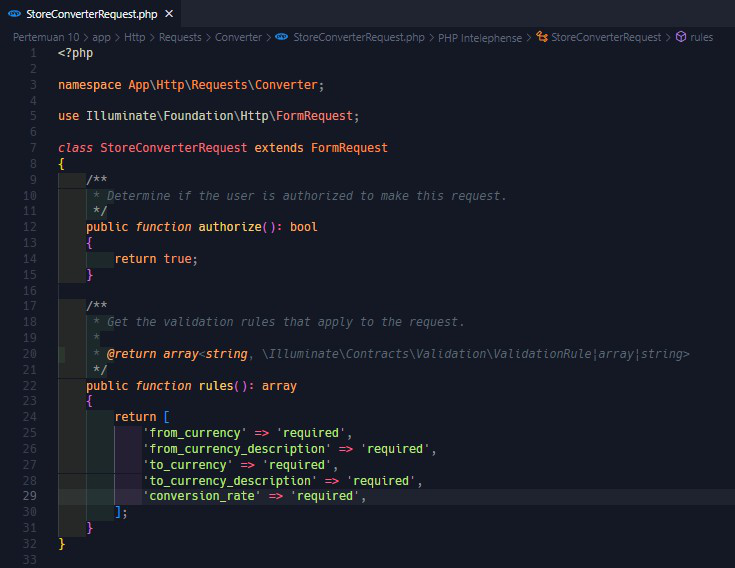
\includegraphics[width=0.6\textwidth]{classFiles/pertemuan-10-request-part-1.png}
 \end{center}
\end{frame}

\begin{frame}[fragile]
 \frametitle{UpdateConverterRequest.php}
 \vskip1cm
 \begin{center}
  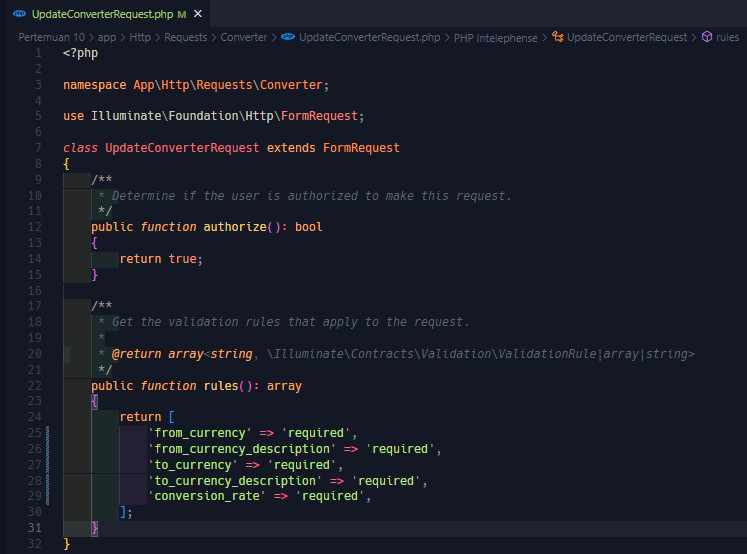
\includegraphics[width=0.6\textwidth]{classFiles/pertemuan-10-request-part-2.png}
 \end{center}
\end{frame}

\begin{frame}[fragile]{Models Converter.php Code Part 1}
\vskip1cm
\begin{lstlisting}[language=PHP]
	<?php
namespace App\Models;
class Converter
{
  // Change the path to the converters.json file
  private static $filePath = 'C:\xampp7\htdocs\pemrograman web\Pertemuan 10\app\Models\converters.json';
public static function all()
  {
    $jsonData = file_get_contents(self::$filePath);
    return collect(json_decode($jsonData, true));
  }
\end{lstlisting}
\end{frame}

\begin{frame}[fragile]{Models Converter Find Function}
\vskip1cm
\begin{lstlisting}[language=PHP]
public static function find(string $id)
  {
    $converters = self::all();
    return $converters->firstWhere('id', $id);
  }
\end{lstlisting}
\end{frame}

\begin{frame}[fragile]{Converter Insert Function Part 1}
\vskip1cm
\begin{lstlisting}[language=PHP]
public static function insert(array $data)
  {
    $converters = self::all();
    $newConverter = [
      'id' => count($converters) + 1,
      'from_currency' => $data['from_currency'],
      'from_currency_description' => $data['from_currency_description'],
      'to_currency' => $data['to_currency'],
      'to_currency_description' => $data['to_currency_description'],
      'conversion_rate' => $data['conversion_rate'],
    ];
\end{lstlisting}
\end{frame}

\begin{frame}[fragile]{Converter Insert Function Part 2}
\vskip1cm
\begin{lstlisting}[language=PHP]
    $convertersArray = $converters->toArray();
    array_push($convertersArray, $newConverter);
    self::saveData($convertersArray);

    return $newConverter;
  }
\end{lstlisting}
\end{frame}

\begin{frame}[fragile]{Converter Update Function Part 1}
\vskip1cm
\begin{lstlisting}[language=PHP]
public static function update(array $data, int $id)
  {
    $converters = self::all();
    $index = collect($converters)->search(function ($item) use ($id) {
      return $item['id'] === $id;
    });
\end{lstlisting}
\end{frame}

\begin{frame}[fragile]{Converter Update Function Part 2}
\vskip1cm
\begin{lstlisting}[language=PHP]
 if ($index !== false) {
      $updatedConverter = [
        'id' => $id,
        'from_currency' => $data['from_currency'],
        'from_currency_description' => $data['from_currency_description'],
        'to_currency' => $data['to_currency'],
        'to_currency_description' => $data['to_currency_description'],
        'conversion_rate' => $data['conversion_rate'],
      ];
\end{lstlisting}
\end{frame}

\begin{frame}[fragile]{Converter Update Function Part 3}
\vskip1cm
\begin{lstlisting}[language=PHP]

      $converters[$index] = $updatedConverter;
      self::saveData($converters);

      return $updatedConverter;
    }

    return null;
  }
\end{lstlisting}
\end{frame}

\begin{frame}[fragile]{Converter Delete Function Part 1}
\vskip1cm
\begin{lstlisting}[language=PHP]
  public static function delete(int $id)
  {
    $converters = self::all();
    $index = collect($converters)->search(function ($item) use ($id) {
      return $item['id'] === $id;
    });

\end{lstlisting}
\end{frame}

\begin{frame}[fragile]{Converter Delete Function Part 2}
\vskip1cm
\begin{lstlisting}[language=PHP]
    if ($index !== false) {
      $convertersArray = $converters->toArray();
      array_splice($convertersArray, $index, 1);
      self::saveData($convertersArray);
      return true;
    }
    return false;
  }
\end{lstlisting}
\end{frame}

\begin{frame}[fragile]{Converter saveData Function}
\vskip1cm
\begin{lstlisting}[language=PHP]
private static function saveData($data)
  {
    file_put_contents(self::$filePath, json_encode($data, JSON_PRETTY_PRINT));
  }
\end{lstlisting}
\end{frame}

\begin{frame}[fragile]
 \frametitle{ConverterController Part 1}
 \vskip1cm
 \begin{center}
  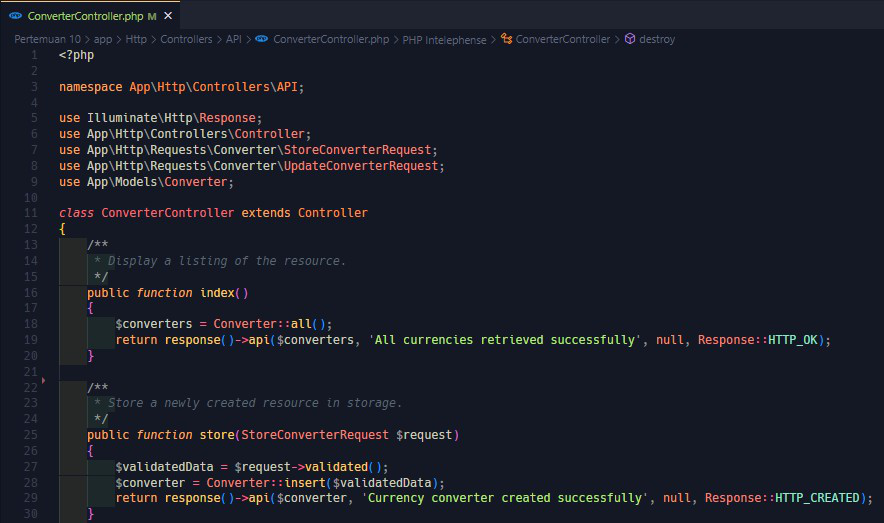
\includegraphics[width=0.6\textwidth]{classFiles/pertemuan-10-controller-part-1.png}
 \end{center}
\end{frame}

\begin{frame}[fragile]
 \frametitle{ConverterController Part 2}
 \vskip1cm
 \begin{center}
  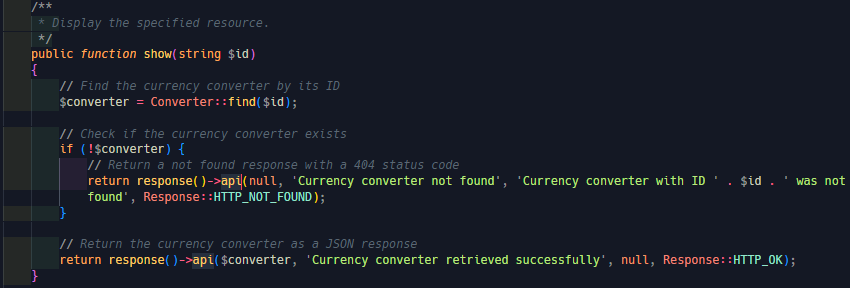
\includegraphics[width=0.6\textwidth]{classFiles/pertemuan-10-controller-part-2.png}
 \end{center}
\end{frame}

\begin{frame}[fragile]
 \frametitle{ConverterController Part 3}
 \vskip1cm
 \begin{center}
  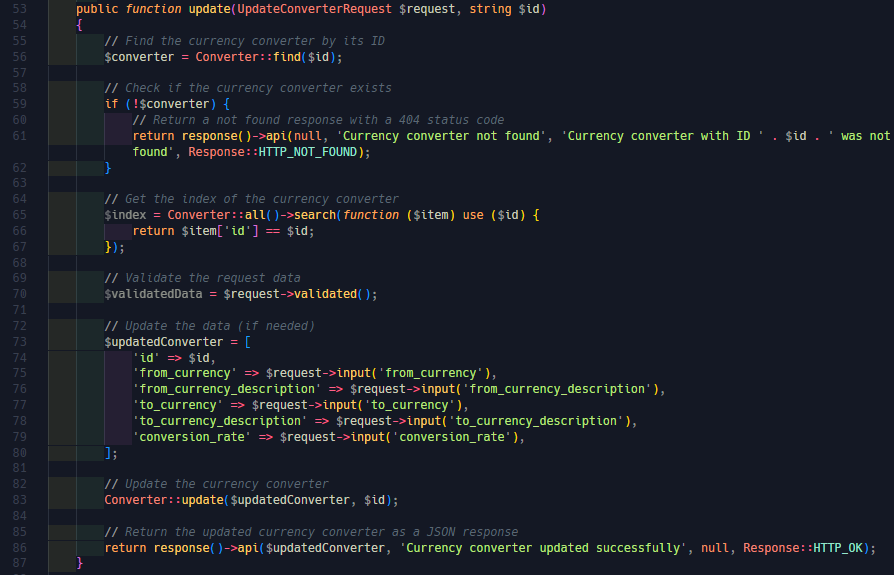
\includegraphics[width=0.6\textwidth]{classFiles/pertemuan-10-controller-part-3.png}
 \end{center}
\end{frame}

\begin{frame}[fragile]
 \frametitle{ConverterController Part 4}
 \vskip1cm
 \begin{center}
  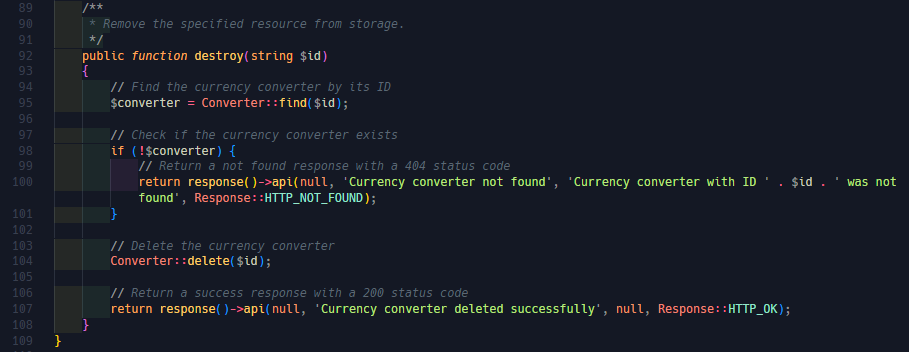
\includegraphics[width=0.6\textwidth]{classFiles/pertemuan-10-controller-part-4.png}
 \end{center}
\end{frame}

\begin{frame}[fragile]
 \frametitle{folder routes/api.php}
 \vskip1cm
 \begin{center}
  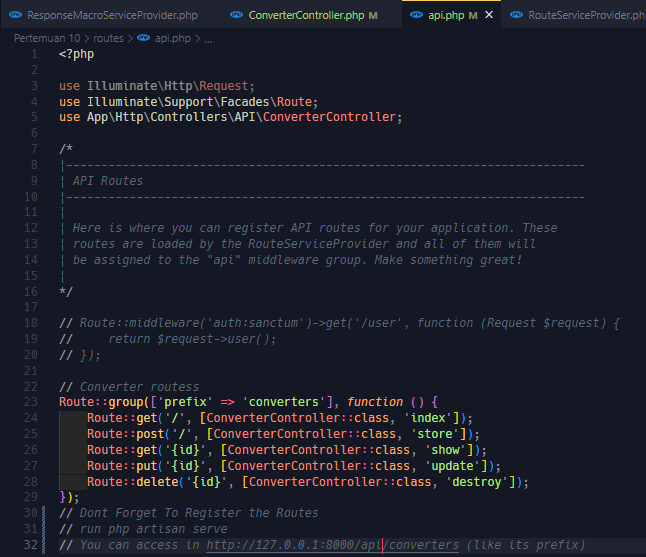
\includegraphics[width=0.6\textwidth]{classFiles/pertemuan-10-routes-api.png}
 \end{center}
\end{frame}

\begin{frame4}
    \frametitle{Thank You}
\end{frame4}

\end{document}
